\chapter*{Problem Statement}
\label{cap:problem-statement}

\addcontentsline{toc}{chapter}{Problem Statement}
\lhead{\bfseries PROBLEM STATEMENT}
\rhead{\thepage}

Il progetto ivi trattato si pone l'obiettivo di progettare e modellare
il comportamento di un insieme di semafori stradali in un'intersezione.
In particolare, si è scelto di riprogettare un semaforo già esistente, 
con lo scopo di migliorarne l'efficienza e la sicurezza. Il semaforo 
scelto a tale scopo è quello presente all'incrocio tra Via del Pomerio, 
Ponte Vanvitelli, Via Posillipo e Corso Vittorio Emanuele III, a Benevento.
Al fine di spiegare meglio la dinamica dell'intersezione, si riportano due 
schermate catturate da Google Maps, che mostrano l'incrocio in questione 
(Fig. \ref{fig:intersection_top} e Fig. \ref{fig:intersection_3d}).

\begin{figure}[H]
    \centering
    \begin{minipage}[b]{.45\textwidth}
        \centering
        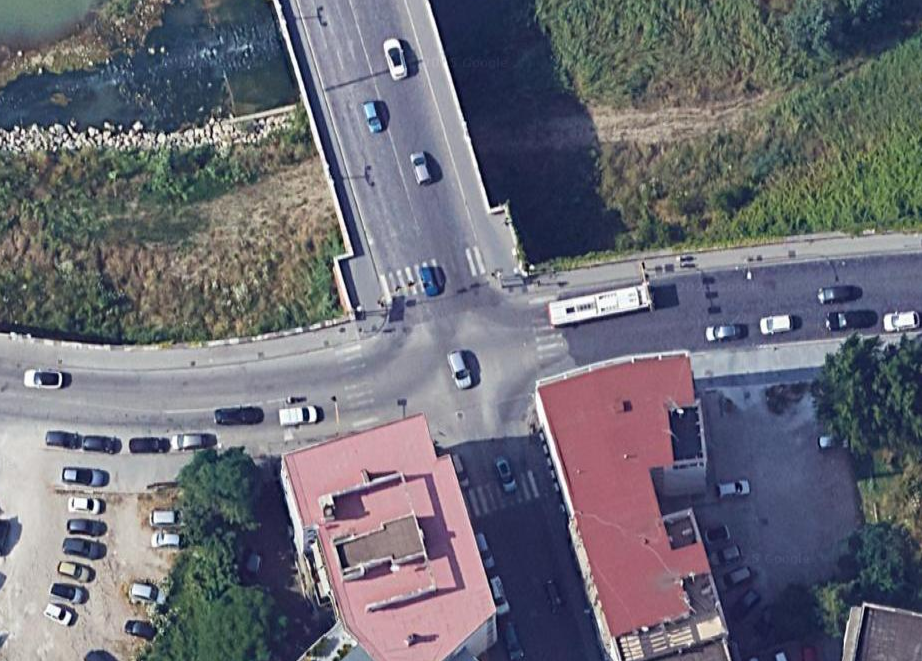
\includegraphics[width=\textwidth]{figure/intersection/incrocio_top.png}
        \caption{Vista dall'alto dell'intersezione}
        \label{fig:intersection_top}
    \end{minipage}
    \hfill
    \begin{minipage}[b]{.45\textwidth}
        \centering
        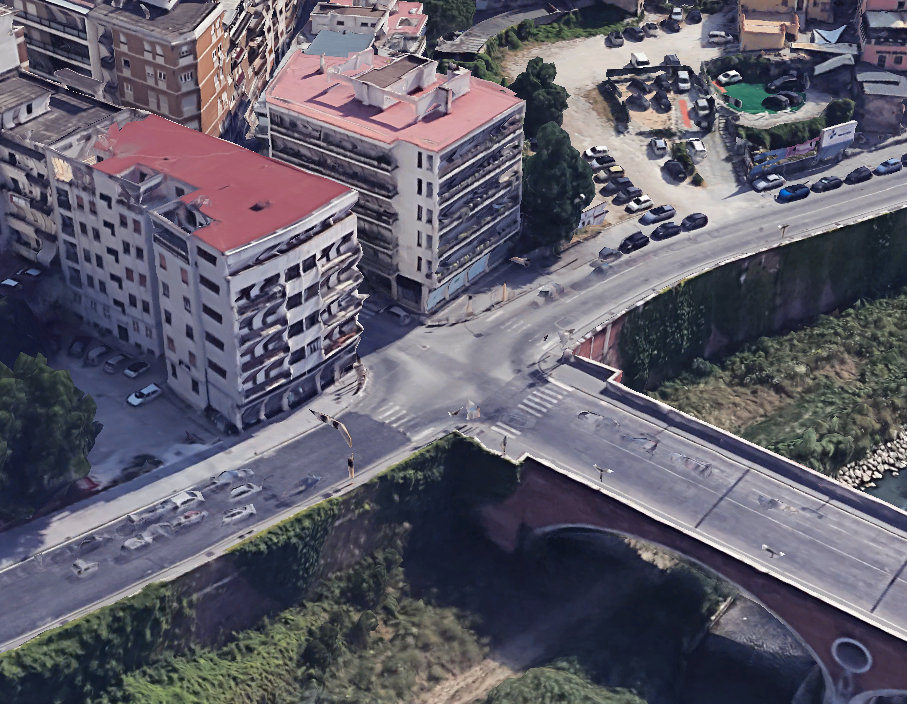
\includegraphics[width=\textwidth]{figure/intersection/incrocio_3d.png}
        \caption{Vista 3D dell'intersezione}
        \label{fig:intersection_3d}
    \end{minipage}
\end{figure}

Come si può quindi dedurre dall'immagine, a Est si trovano tre semafori 
che consentono di andare a Nord, Sud e Ovest. A Ovest, invece, si trovano 
due semafori che consentono di andare a Nord e a Sud. Il semaforo a Nord, 
infine, consente di andare a Ovest o a Sud. Ogni combinazione provenienza-destinazione 
si trova su un'apposita corsia e ha un semaforo dedicato.

Al fine di modellare il comportamento del semaforo, si è scelto di utilizzare 
il formalismo delle Reti di Petri, in quanto permette di modellare sistemi 
concorrenti e distribuiti in modo chiaro e intuitivo. Nel caso modellato, 
per migliorare l'efficienza del semaforo, si è scelto di permettere il 
passaggio di più veicoli contemporaneamente, qualora possibile, imponendo 
vincoli per evitare che due o più veicoli si incrocino. Ad esempio è consentito 
il passaggio contemporaneo di un veicolo proveniente da Est diretto verso Nord 
e uno proveniente da Ovest e diretto verso Sud. Al contrario, invece, non è possibile 
attraversare contemporaneamente l'incrocio con due veicoli provenienti da direzioni diverse 
e diretti nella stessa direzione, in quanto ciò potrebbe causare un incidente. Inoltre, 
non è possibile che due veicoli si incontrino all'interno dell'incrocio, come ad esempio 
un veicolo che attraversa l'incrocio da Est a Ovest e un veicolo che attraversa l'incrocio da Nord a Sud.

Tali vincoli sono stati modellati con l'utilizzo di GMEC, come mostrato nelle sezioni successive.